% The code is quite messy !!!

\documentclass[tikz,border=10pt]{standalone}

\definecolor{darkgreen}{rgb}{0,0.5,0}

\begin{document}

    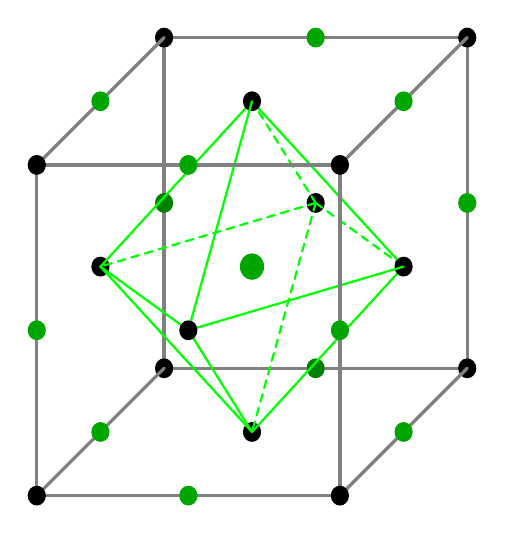
\begin{tikzpicture}[scale=3.5, x={(1.1,0)}, y={(0,1.2)}, z={(0, 0, 1.2)}, line join=round, line cap=round]

        % Cube edges
        \draw[gray, very thick] (0,0,0) -- (1,0,0) -- (1,1,0) -- (0,1,0) -- cycle; % face du fond

        % Vertices of the cube (background)
        \foreach \x/\y/\z in {0/0/0, 1/0/0, 1/1/0, 0/1/0, 0.5/0.5/0, 0/0.5/0.5, 0.5/0/0.5} {
            \fill[black] (\x,\y,\z) circle (0.03);
        }

    
        \fill[darkgreen!70!green] (0.5,0.5,0.5) circle (0.04);
    

        % Octahedral site (green) (background)
        \foreach \x/\y/\z in {0.5/0/0, 0/0.5/0} {
            \fill[darkgreen] (\x, \y, \z) circle (0.03);
        }

        % aretes sites octa
        \draw[green, thick, dotted][dash pattern=on 1mm off 0.8mm] (0.5,0.5,0) -- (0.5,0,0.5); % face de derriere
        \draw[green, thick, dotted][dash pattern=on 1mm off 0.8mm] (0.5,0.5,0) -- (0.5,1,0.5);
        \draw[green, thick, dotted][dash pattern=on 1mm off 0.8mm] (0.5,0.5,0) -- (0,0.5,0.5);
        \draw[green, thick, dotted][dash pattern=on 1mm off 0.8mm] (0.5,0.5,0) -- (1,0.5,0.5);

        \draw[green, thick] (0.5,1,0.5) -- (1,0.5,0.5); % entre noeud faces
        \draw[green, thick] (1,0.5,0.5) -- (0.5,0,0.5); % entre noeud faces
        \draw[green, thick] (0.5,0,0.5) -- (0,0.5,0.5); % entre noeud faces
        \draw[green, thick] (0.5,1,0.5) -- (0,0.5,0.5); % entre noeud faces
        
        % cube top face verteses and right face
        \fill[black] (0.5,1,0.5) circle (0.03);
        \fill[black] (1,0.5,0.5) circle (0.03);
        
        % entre noeud face avant
        \draw[green, thick] (0.5,0.5,1) -- (0.5,0,0.5); % face de devant
        \draw[green, thick] (0.5,0.5,1) -- (0.5,1,0.5);
        \draw[green, thick] (0.5,0.5,1) -- (0,0.5,0.5);
        \draw[green, thick] (0.5,0.5,1) -- (1,0.5,0.5);
        
        % cube aretes
        \draw[gray, very thick] (0,0,0) -- (0,0,1); 
        \draw[gray, very thick] (1,0,0) -- (1,0,1);
        \draw[gray, very thick] (1,1,0) -- (1,1,1);
        \draw[gray, very thick] (0,1,0) -- (0,1,1);
        \draw[gray, very thick] (0,0,1) -- (1,0,1) -- (1,1,1) -- (0,1,1) -- cycle; % face avant

        % Octahedral site (green)
        \foreach \x/\y/\z in {0.5/1/0, 0.5/0/1, 0.5/1/1, 1/0.5/0, 0/0.5/1, 1/0.5/1, 0/0/0.5, 1/0/0.5, 0/1/0.5, 1/1/0.5} {
            \fill[darkgreen!70!green] (\x, \y, \z) circle (0.03);
        }

        % Vertices of the cube (foreground)
        \foreach \x/\y/\z in {0/0/1, 1/0/1, 1/1/1, 0/1/1, 0.5/0.5/1} {
            \fill[black] (\x,\y,\z) circle (0.03);
        }

    \end{tikzpicture}

\end{document}